%10_adverserial_search.tex
%notes for the course PandA2 COMS10001 taught at the University of Bristol
%2016-7 Conor Houghton conor.houghton@bristol.ac.uk

%To the extent possible under law, the author has dedicated all copyright 
%and related and neighboring rights to these notes to the public domain 
%worldwide. These notes are distributed without any warranty. 

\documentclass[11pt,a4paper]{scrartcl}
\typearea{12}
\usepackage{graphicx}
\usepackage{listings}
\usepackage{tikz-qtree}
\lstset{language=C}
\pagestyle{headings}
\markright{COMS10001 - PandA2 10\_adverserial\_search - Conor}
\begin{document}

\subsection*{10 - adverserial search}


\subsubsection*{Nim example}

Nim is a simple game using counters for two players; the counters are
divided into some number of piles and the players take turns removing
counters. In a go a player must take at least one counter and can take
as many counters as they like, provided they only come from one
pile. Thus, in each go each player removes counters from only one
pile. The winner is the player who takes the last piece. An example game is given in Table~\ref{tab:nim_example}

\begin{table}
\begin{tabular}{cccc|l}
5&2&6&3&Initial arrangement\\
1&2&6&3&\textbf{A}oife takes four from pile one\\
1&2&6&0&\textbf{B}rendan takes three from pile four\\
1&2&1&0&\textbf{A}oife takes five from pile three\\
1&1&1&0&\textbf{B}rendan takes one from pile two\\
1&0&1&0&\textbf{A}oife takes one from pile two\\
1&0&0&0&\textbf{B}rendan takes one from pile two\\
0&0&0&0&\textbf{A}oife takes one from pile one and wins
\end{tabular}
\caption{An example of two players playing nim; this illustrates game play, neither player is playing optimally. The four columns give the number of counters in the four piles directly after the move described in the same row.\label{tab:nim_example}}
\end{table}

Nim can be enjoyable to play, but it is mostly beloved of
mathematicians and computer scientists because it is a good example in
explanations like this one and because it was solved as a game, for
all numbers of piles and counters, in 1902 by Charles L. Bouton, in a
paper which is to have founded combinatorial game theory. What we are
interested in here stops short of solving the game analytically,
instead in Fig.~\ref{fig:nim} we map out a tree giving all possible
moves for nim with three piles of two. Thus, from the initial
configuration $(2,2,2)$ leaving out alternatives that are equivalent
to each other, there are two possible moves, the player can take one
or two counters from one of the piles, leading to $(1,2,2)$ or
$(0,2,2)$. From $(1,2,2)$ there are then three alternatives, leading
to $(0,1,2)$, $(1,1,2)$ and $(0,2,2)$, and so on.

Now the leaves of the tree all have two zeros, who ever has the next
move wins. This means we can score the leaves; for definateness lets
imagine the human player has the first go, we will score +1 for leaves
where the human player has the next go, -1 if the computer does. This
is shown in Fig.~\ref{fig:nim-leaves}; the problem is that the leaves
are far removed from the current move, the human player is at
$(2,2,2)$ and decided between $(1,2,2)$ and $(0,2,2)$; we need to move
the scoring up from the leaves to the root.

\begin{figure}
\begin{center}
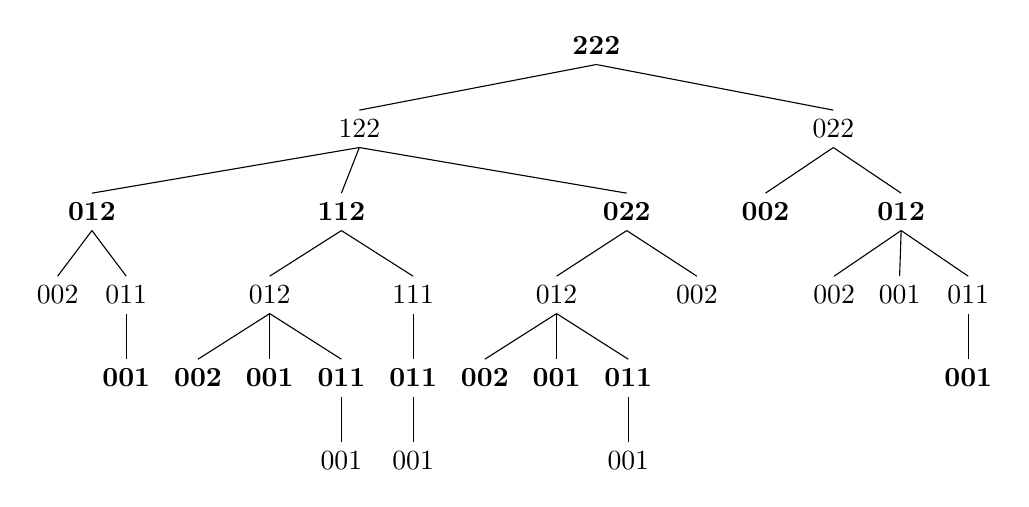
\begin{tikzpicture}
\Tree
[.\textbf{222}   
  [.122
    [.\textbf{012} 
      [.002 ]
      [.011 \textbf{001} ]
    ]
    [.\textbf{112} 
      [.012
        [.\textbf{002} ]
        [.\textbf{001} ]
        [.\textbf{011} 001 ]
      ]
      [.111
        [.\textbf{011} 001 ]
      ]
    ]
    [.\textbf{022} 
      [.012
        [.\textbf{002} ]
        [.\textbf{001} ]
        [.\textbf{011} 001 ]
      ]
      [.002 ]
    ]
  ]
  [.022
    [.\textbf{002} ]
    [.\textbf{012} 
      [.002 ]
      [.001 ]
      [.011 \textbf{001} ]
    ]
  ]
]
\end{tikzpicture}
\end{center}
\caption{The whole game tree for nim starting with $(2,2,2)$; some
  equivalent choices have been left out, so it includes $(1,2,2)$ on
  the second ply, but not $(2,1,2)$; for clarity the triples are
  arranges in ascending order. Alternative ply are bolded to help keep
  track of who is playing, if the human player goes first he or she is
  bold, whereas her or his computer opponent is
  unbolded. \label{fig:nim}}
\end{figure}

\begin{figure}
\begin{center}
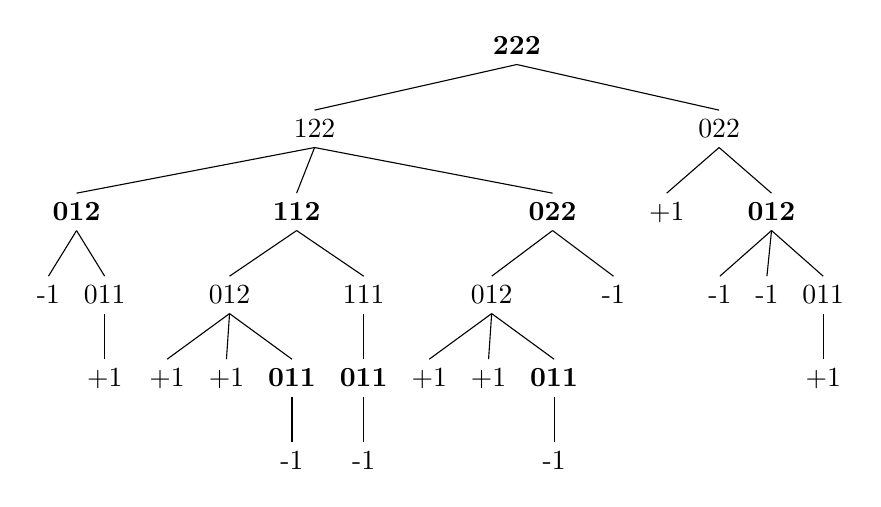
\begin{tikzpicture}
\Tree
[.\textbf{222}   
  [.122
    [.\textbf{012} 
      [.-1 ]
      [.011 +1 ]
    ]
    [.\textbf{112} 
      [.012
        [.+1 ]
        [.+1 ]
        [.\textbf{011} -1 ]
      ]
      [.111
        [.\textbf{011} -1 ]
      ]
    ]
    [.\textbf{022} 
      [.012
        [.+1 ]
        [.+1 ]
        [.\textbf{011} -1 ]
      ]
      [.-1 ]
    ]
  ]
  [.022
    [.+1 ]
    [.\textbf{012} 
      [.-1 ]
      [.-1 ]
      [.011 +1 ]
    ]
  ]
]
\end{tikzpicture}
\end{center}
\caption{Here the leaves have been scored, +1 for a human win, -1 if the computer wins. Since each player takes just one move in each turn, it is easy to score the leaves, the bold ones go to +1, the unbolded to -1.\label{fig:nim-leaves}}
\end{figure}






\begin{figure}
\begin{center}
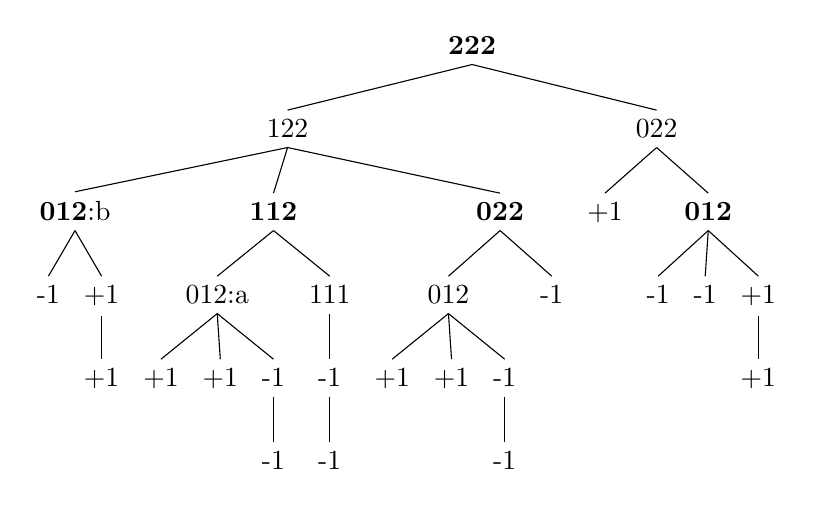
\begin{tikzpicture}
\Tree
[.\textbf{222}   
  [.122
    [.\textbf{012}:b 
      [.-1 ]
      [.+1 +1 ]
    ]
    [.\textbf{112} 
      [.012:a
        [.+1 ]
        [.+1 ]
        [.-1 -1 ]
      ]
      [.111
        [.-1 -1 ]
      ]
    ]
    [.\textbf{022} 
      [.012
        [.+1 ]
        [.+1 ]
        [.-1 -1 ]
      ]
      [.-1 ]
    ]
  ]
  [.022
    [.+1 ]
    [.\textbf{012} 
      [.-1 ]
      [.-1 ]
      [.+1 +1 ]
    ]
  ]
]
\end{tikzpicture}
\end{center}
\caption{\label{fig:nim-leaves_1}}
\end{figure}


\begin{figure}
\begin{center}
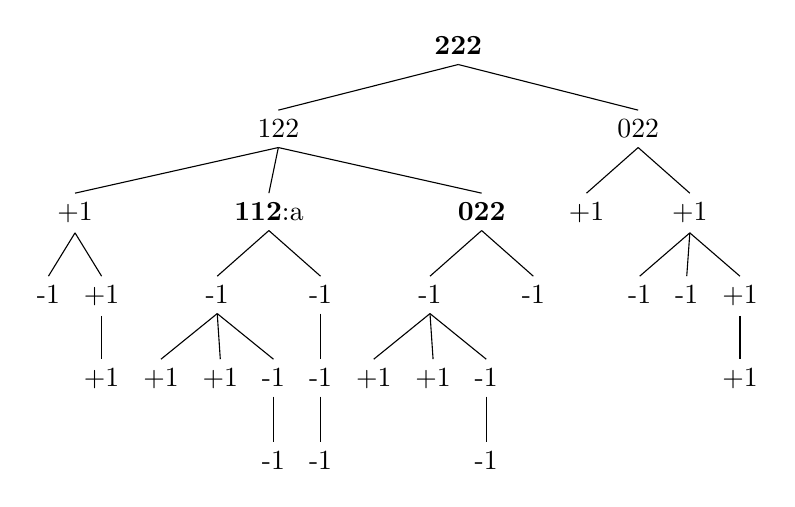
\begin{tikzpicture}
\Tree
[.\textbf{222}   
  [.122
    [.+1 
      [.-1 ]
      [.+1 +1 ]
    ]
    [.\textbf{112}:a 
      [.-1
        [.+1 ]
        [.+1 ]
        [.-1 -1 ]
      ]
      [.-1
        [.-1 -1 ]
      ]
    ]
    [.\textbf{022} 
      [.-1
        [.+1 ]
        [.+1 ]
        [.-1 -1 ]
      ]
      [.-1 ]
    ]
  ]
  [.022
    [.+1 ]
    [.+1 
      [.-1 ]
      [.-1 ]
      [.+1 +1 ]
    ]
  ]
]
\end{tikzpicture}
\end{center}
\caption{\label{fig:nim-leaves_2}}
\end{figure}


\begin{figure}
\begin{center}
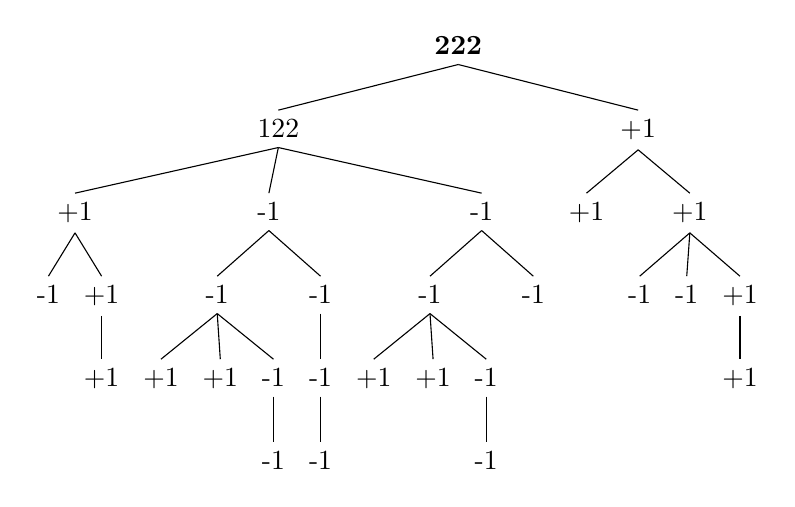
\begin{tikzpicture}
\Tree
[.\textbf{222}   
  [.122
    [.+1 
      [.-1 ]
      [.+1 +1 ]
    ]
    [.-1
      [.-1
        [.+1 ]
        [.+1 ]
        [.-1 -1 ]
      ]
      [.-1
        [.-1 -1 ]
      ]
    ]
    [.-1 
      [.-1
        [.+1 ]
        [.+1 ]
        [.-1 -1 ]
      ]
      [.-1 ]
    ]
  ]
  [.+1
    [.+1 ]
    [.+1 
      [.-1 ]
      [.-1 ]
      [.+1 +1 ]
    ]
  ]
]
\end{tikzpicture}
\end{center}
\caption{\label{fig:nim-leaves_3}}
\end{figure}


\begin{figure}
\begin{center}
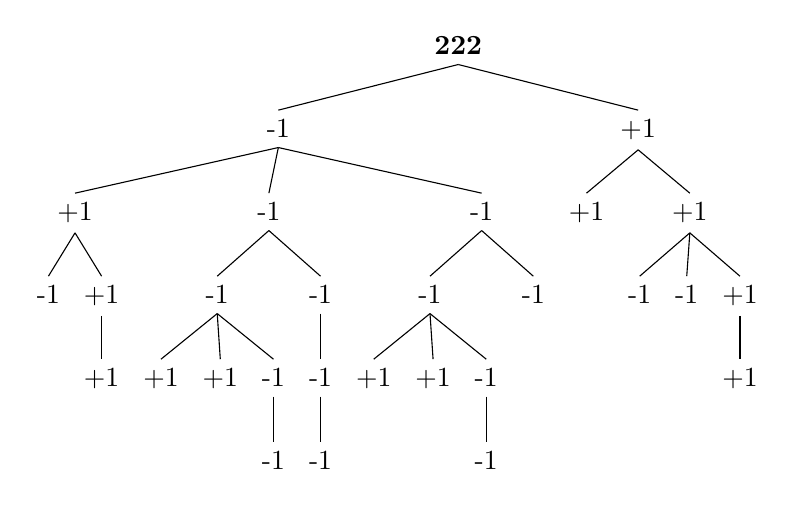
\begin{tikzpicture}
\Tree
[.\textbf{222}   
  [.-1
    [.+1 
      [.-1 ]
      [.+1 +1 ]
    ]
    [.-1
      [.-1
        [.+1 ]
        [.+1 ]
        [.-1 -1 ]
      ]
      [.-1
        [.-1 -1 ]
      ]
    ]
    [.-1 
      [.-1
        [.+1 ]
        [.+1 ]
        [.-1 -1 ]
      ]
      [.-1 ]
    ]
  ]
  [.+1
    [.+1 ]
    [.+1 
      [.-1 ]
      [.-1 ]
      [.+1 +1 ]
    ]
  ]
]
\end{tikzpicture}
\end{center}
\caption{\label{fig:nim-leaves_4}}
\end{figure}


\end{document}
